\documentclass{article}
	\usepackage[utf8]{inputenc}
	\usepackage{float}
	\usepackage{pdfpages}
	\usepackage[T1]{fontenc}
	\usepackage{float}
	\usepackage{booktabs}
	\usepackage{multirow}
	\usepackage{ragged2e}
	\usepackage{makecell}
	\renewcommand{\theadfont}{\small\bfseries}
	\usepackage{tabularx}
	\usepackage[autolanguage, np]{numprint}
	\newcolumntype{Z}{ >{\centering\arraybackslash}X }
	\usepackage{makecell}
	\usepackage{url}
	\usepackage{siunitx}
	\usepackage{caption}
	\usepackage[framemethod=TikZ]{mdframed}
	\usepackage{tikz, tabularx}
	\usepackage[T1]{fontenc}
	\usepackage{charter}

%%% Document Properties and Packages used 9/20
\usepackage{amsmath}        % math formulas
\usepackage{bm}             % bold math symbols
\usepackage{multicol}       % multiple columns
\usepackage[super]{nth}     % 1st, 2nd, 3rd, 4th
\usepackage{enumitem}       % ordered list (a), (b), (c)
\usepackage{graphicx}		% insert images
\graphicspath{ {./images/} }
\usepackage{geometry}
\geometry{letterpaper, margin=1in, top=0.5in} % small margins
%\usepackage{biblatex}		% bibliography
%\addbibresource{HW1N1.bib}
%%%%%%%%%%%%%%%%%%%%%%%%%%%%%%%%%%%%%%%%%%%%%%%%%%%%%%%%%%%%%%%%%%%%%%%%%%%%%%%
%%% Code Listing 
\usepackage{listings}
\usepackage{xcolor}

\definecolor{codegreen}{rgb}{0,0.6,0}
\definecolor{codegray}{rgb}{0.5,0.5,0.5}
\definecolor{codepurple}{rgb}{0.58,0,0.82}
\definecolor{backcolour}{rgb}{0.95,0.95,0.92}

\lstdefinestyle{mystyle}{
	backgroundcolor=\color{backcolour},   
	commentstyle=\color{codegreen},
	keywordstyle=\color{magenta},
	numberstyle=\tiny\color{codegray},
	stringstyle=\color{codepurple},
	basicstyle=\ttfamily\footnotesize,
	breakatwhitespace=false,         
	breaklines=true,                 
	captionpos=b,                    
	keepspaces=true,                 
	numbers=left,                    
	numbersep=5pt,                  
	showspaces=false,                
	showstringspaces=false,
	showtabs=false,                  
	tabsize=2
}
\lstset{style=mystyle}
%%%%%%%%%%%%%%%%%%%%%%%%%%%%%%%%%%%%%%%%%%%%%%%%%%%%%%%%%%%%%%%%%%%%%%%%%%%%%%%
\begin{document}
	
	\noindent\textbf{Justine John "JJ" A. Serdoncillo}
	\hfill \textbf{EE 5571: Reinforcement Learning and Dynamic Programming} \\ \hfill \textbf{December 5, 2023}
    \hfill \textbf{Tuesday}
	
	\begin{center}
		\Large{\textbf{Traveling Salesman Extreme Version}} 
	\end{center}
	
	\section*{Problem Statement}
    Consider the distance matrix provided in the file HW6Data. Your goal is to find a route of the Traveling Salesperson for this matrix assuming you start and finish your tour at node 1. In a tour you can only visit each city once, and the tour is complete once you have visited all cities. Your goal is to minimize your total distance traveled. You will use rollout with a base policy of nearest neighbor to find your route.

    \section*{Solutions}
        Based from the plot that I was able to produce, it can be seen that with the fixed epsilon, the performance using SARSA is different from the other two methods. 
        However, it can be seen that once the Variable Epsilon is used, the performances are roughly the same for all the different methods.
            \begin{figure}[H]
				\centering
				%%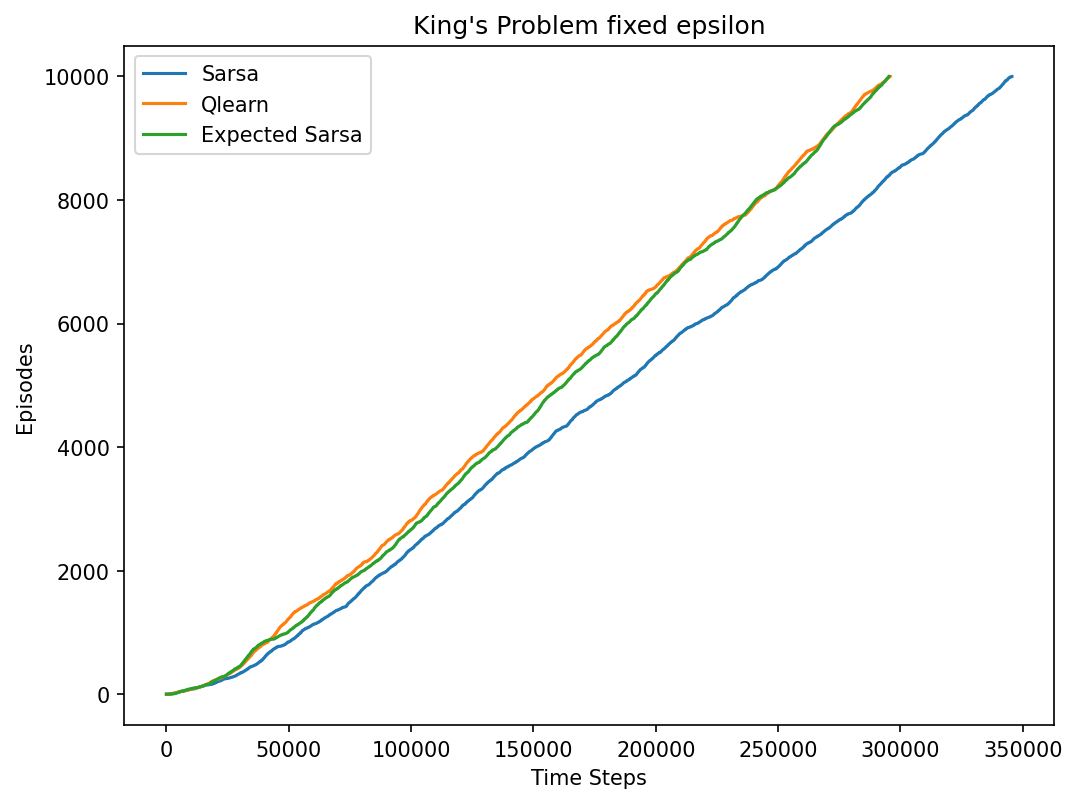
\includegraphics[width=0.5\textwidth]{images/first.png}
				\caption{ Fixed Epsilon }
			\end{figure}
            \begin{figure}[H]
				\centering
				%%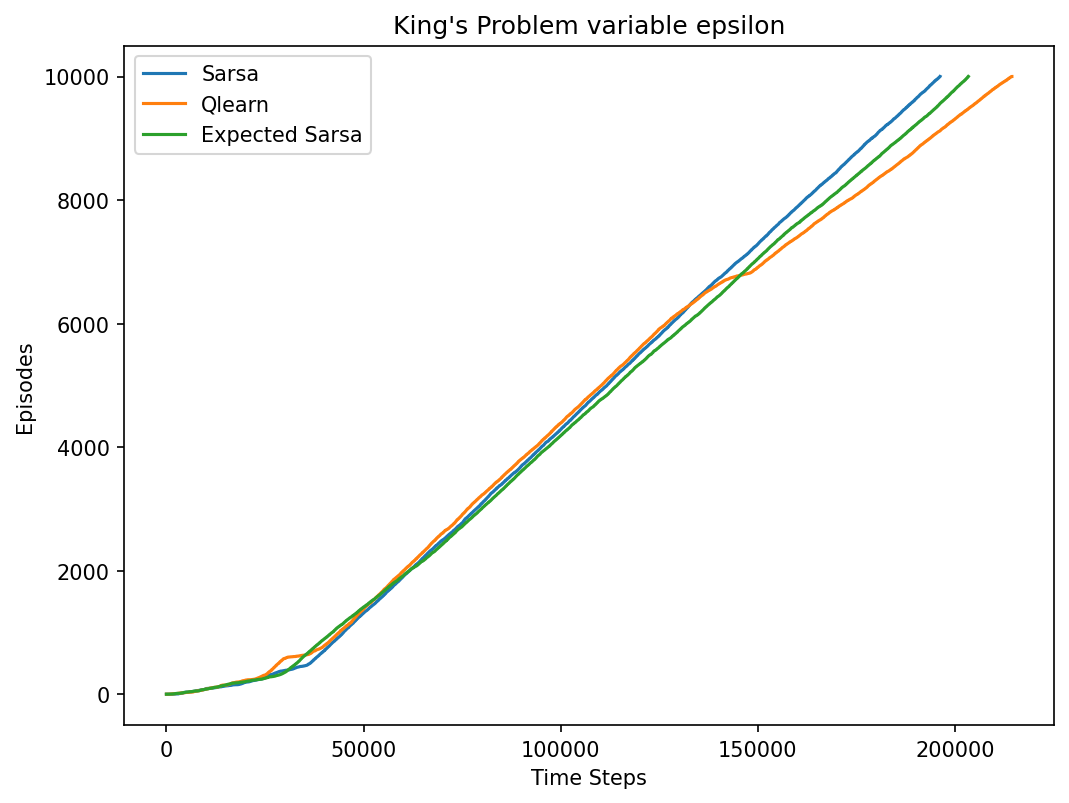
\includegraphics[width=0.5\textwidth]{images/second.png}
				\caption{ Variable Epsilon }
			\end{figure}
   
                    
		\newpage
		\section*{Appendix}
			\subsection*{ Python }
			%% \lstinputlisting[language=Python]{hw4_exer6_10.py}
			
\end{document}
